\subsection{Airy and Pratt hypothesis for mountain ranges}
\textbf{(a)}
\begin{center}
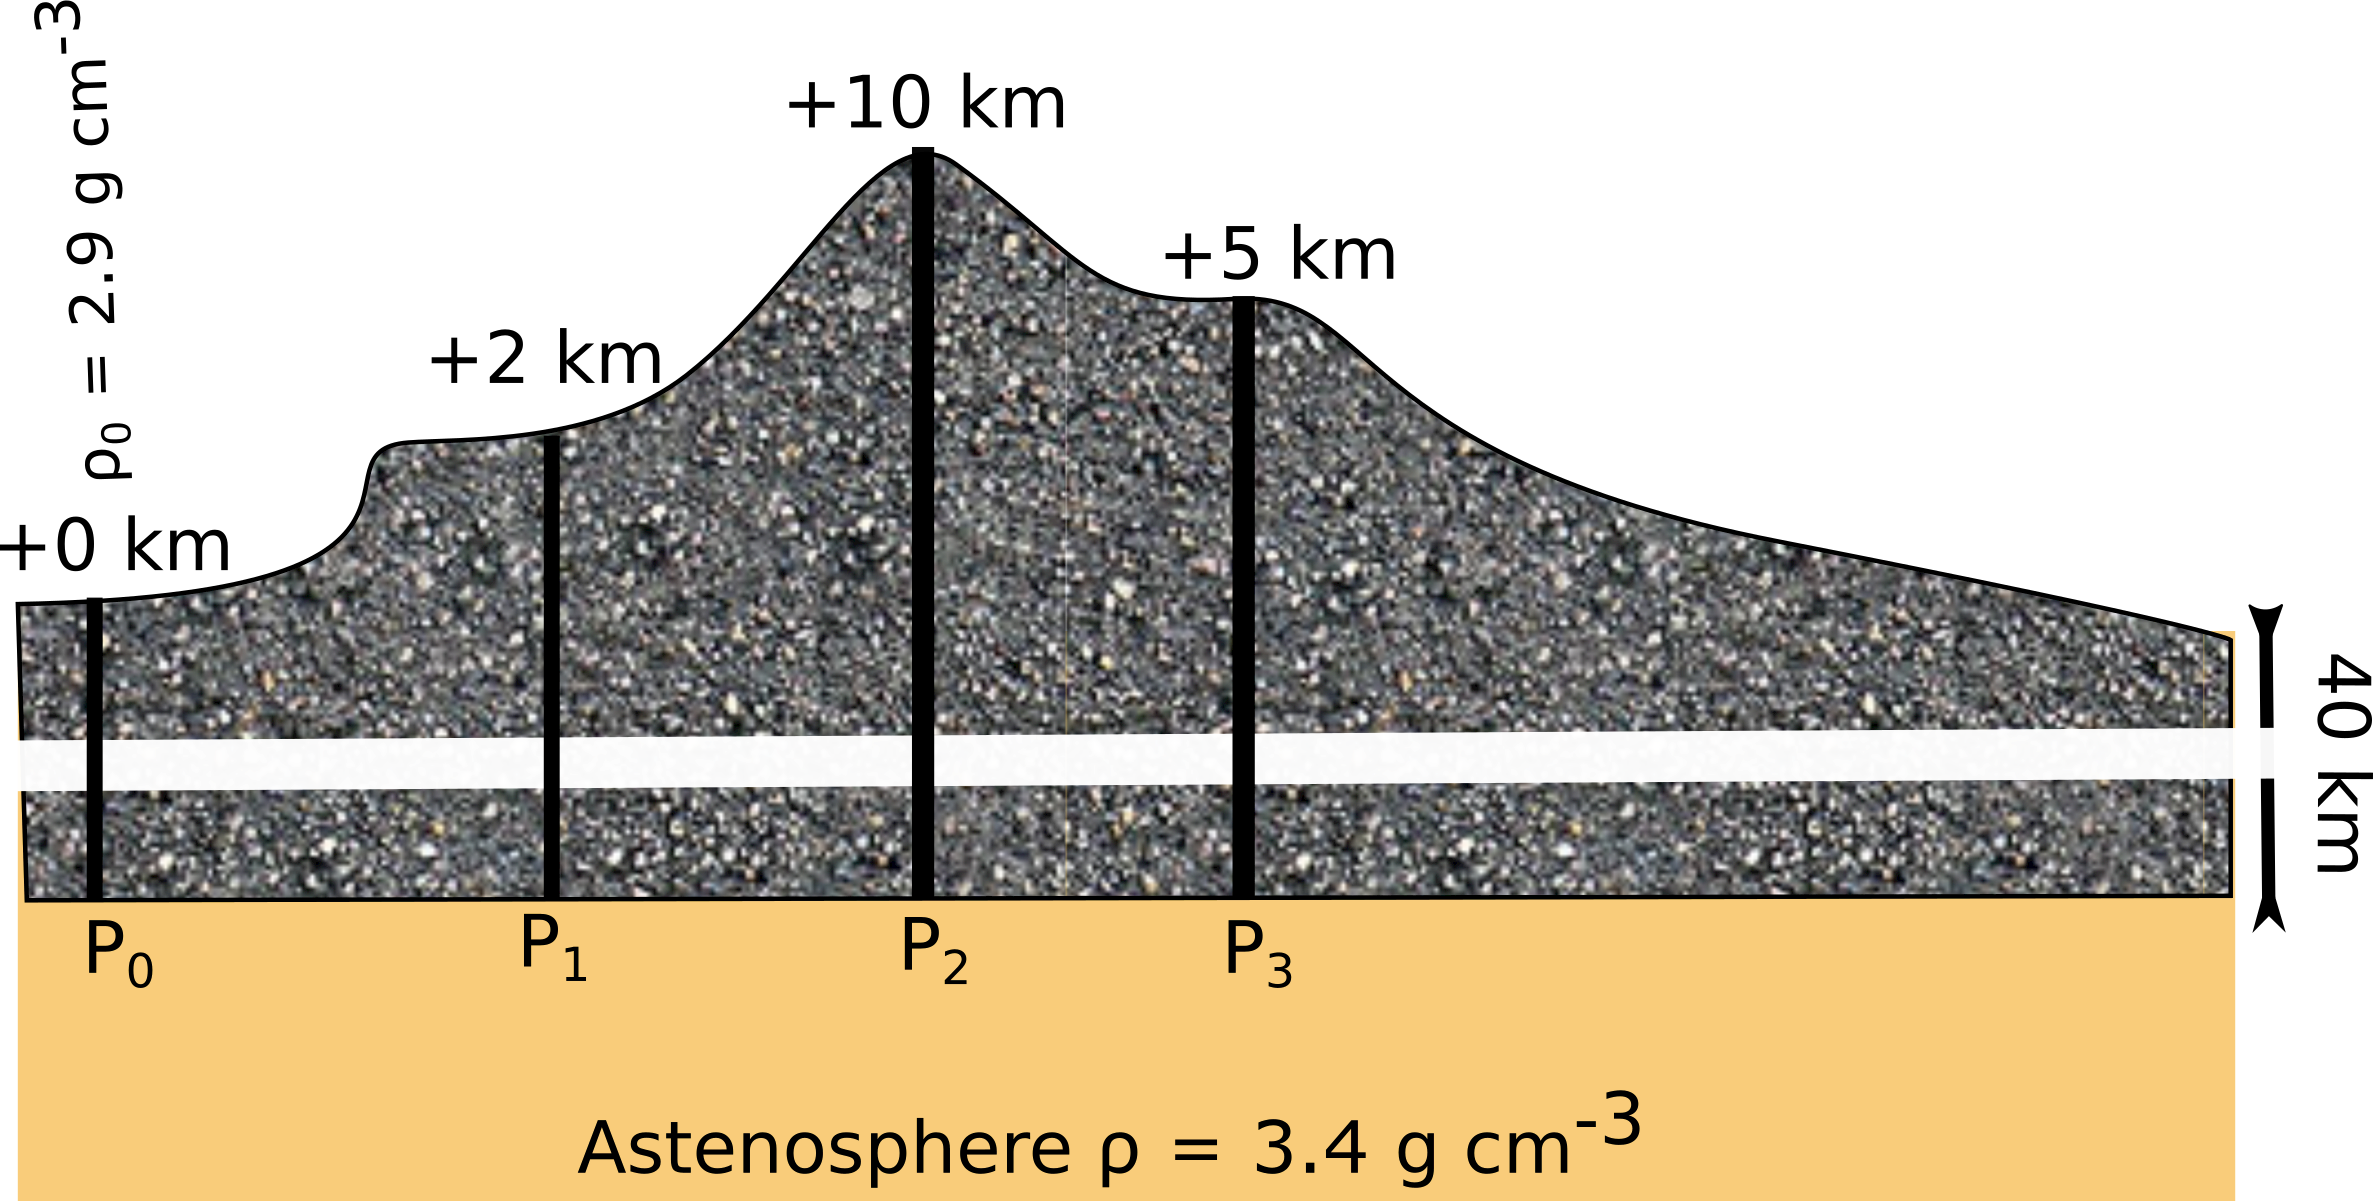
\includegraphics[width=0.5\textwidth]{Figures/Gravimetry/Pratt.png}
\end{center}

The figure above illustrates a crust with  with a inhomogenous density and a mountain change floating on the asthenosphere. Consider this as an idealised case in which every vertical slice is locally balanced (i.e. everything is in hydrostatic equilibrium which reduces to an effective 1D problem). Calculate the required densities in the vertical slices at $P_1 -- P_3$. (Tip: Below the crust the pressure is equal everywhere $P_1 -- P_3$)


\ifanswers
  \begin{tcolorbox}[enhanced jigsaw,breakable,pad at break*=1mm,
    colback=blue!5!white,colframe=babyblueeyes,title=Solutions]
The hydrostatic pressure $p$ at $P_1$ is $p ~ \rho g H_1$ with $H_1=40$~km. This is the same for the other locations. Hence:
\begin{align*}
\rho_0 H_1 &= \rho_1 (H_1 + 2) \\
\rightarrow \rho_1 &= \rho_0 \frac{H_1}{H_1+2} \approx 2.76 \, \text{g cm}^{-3}
\end{align*}
Equivalent for the other locations.
\end{tcolorbox}
\fi
\textbf{(b)}
\begin{center}
  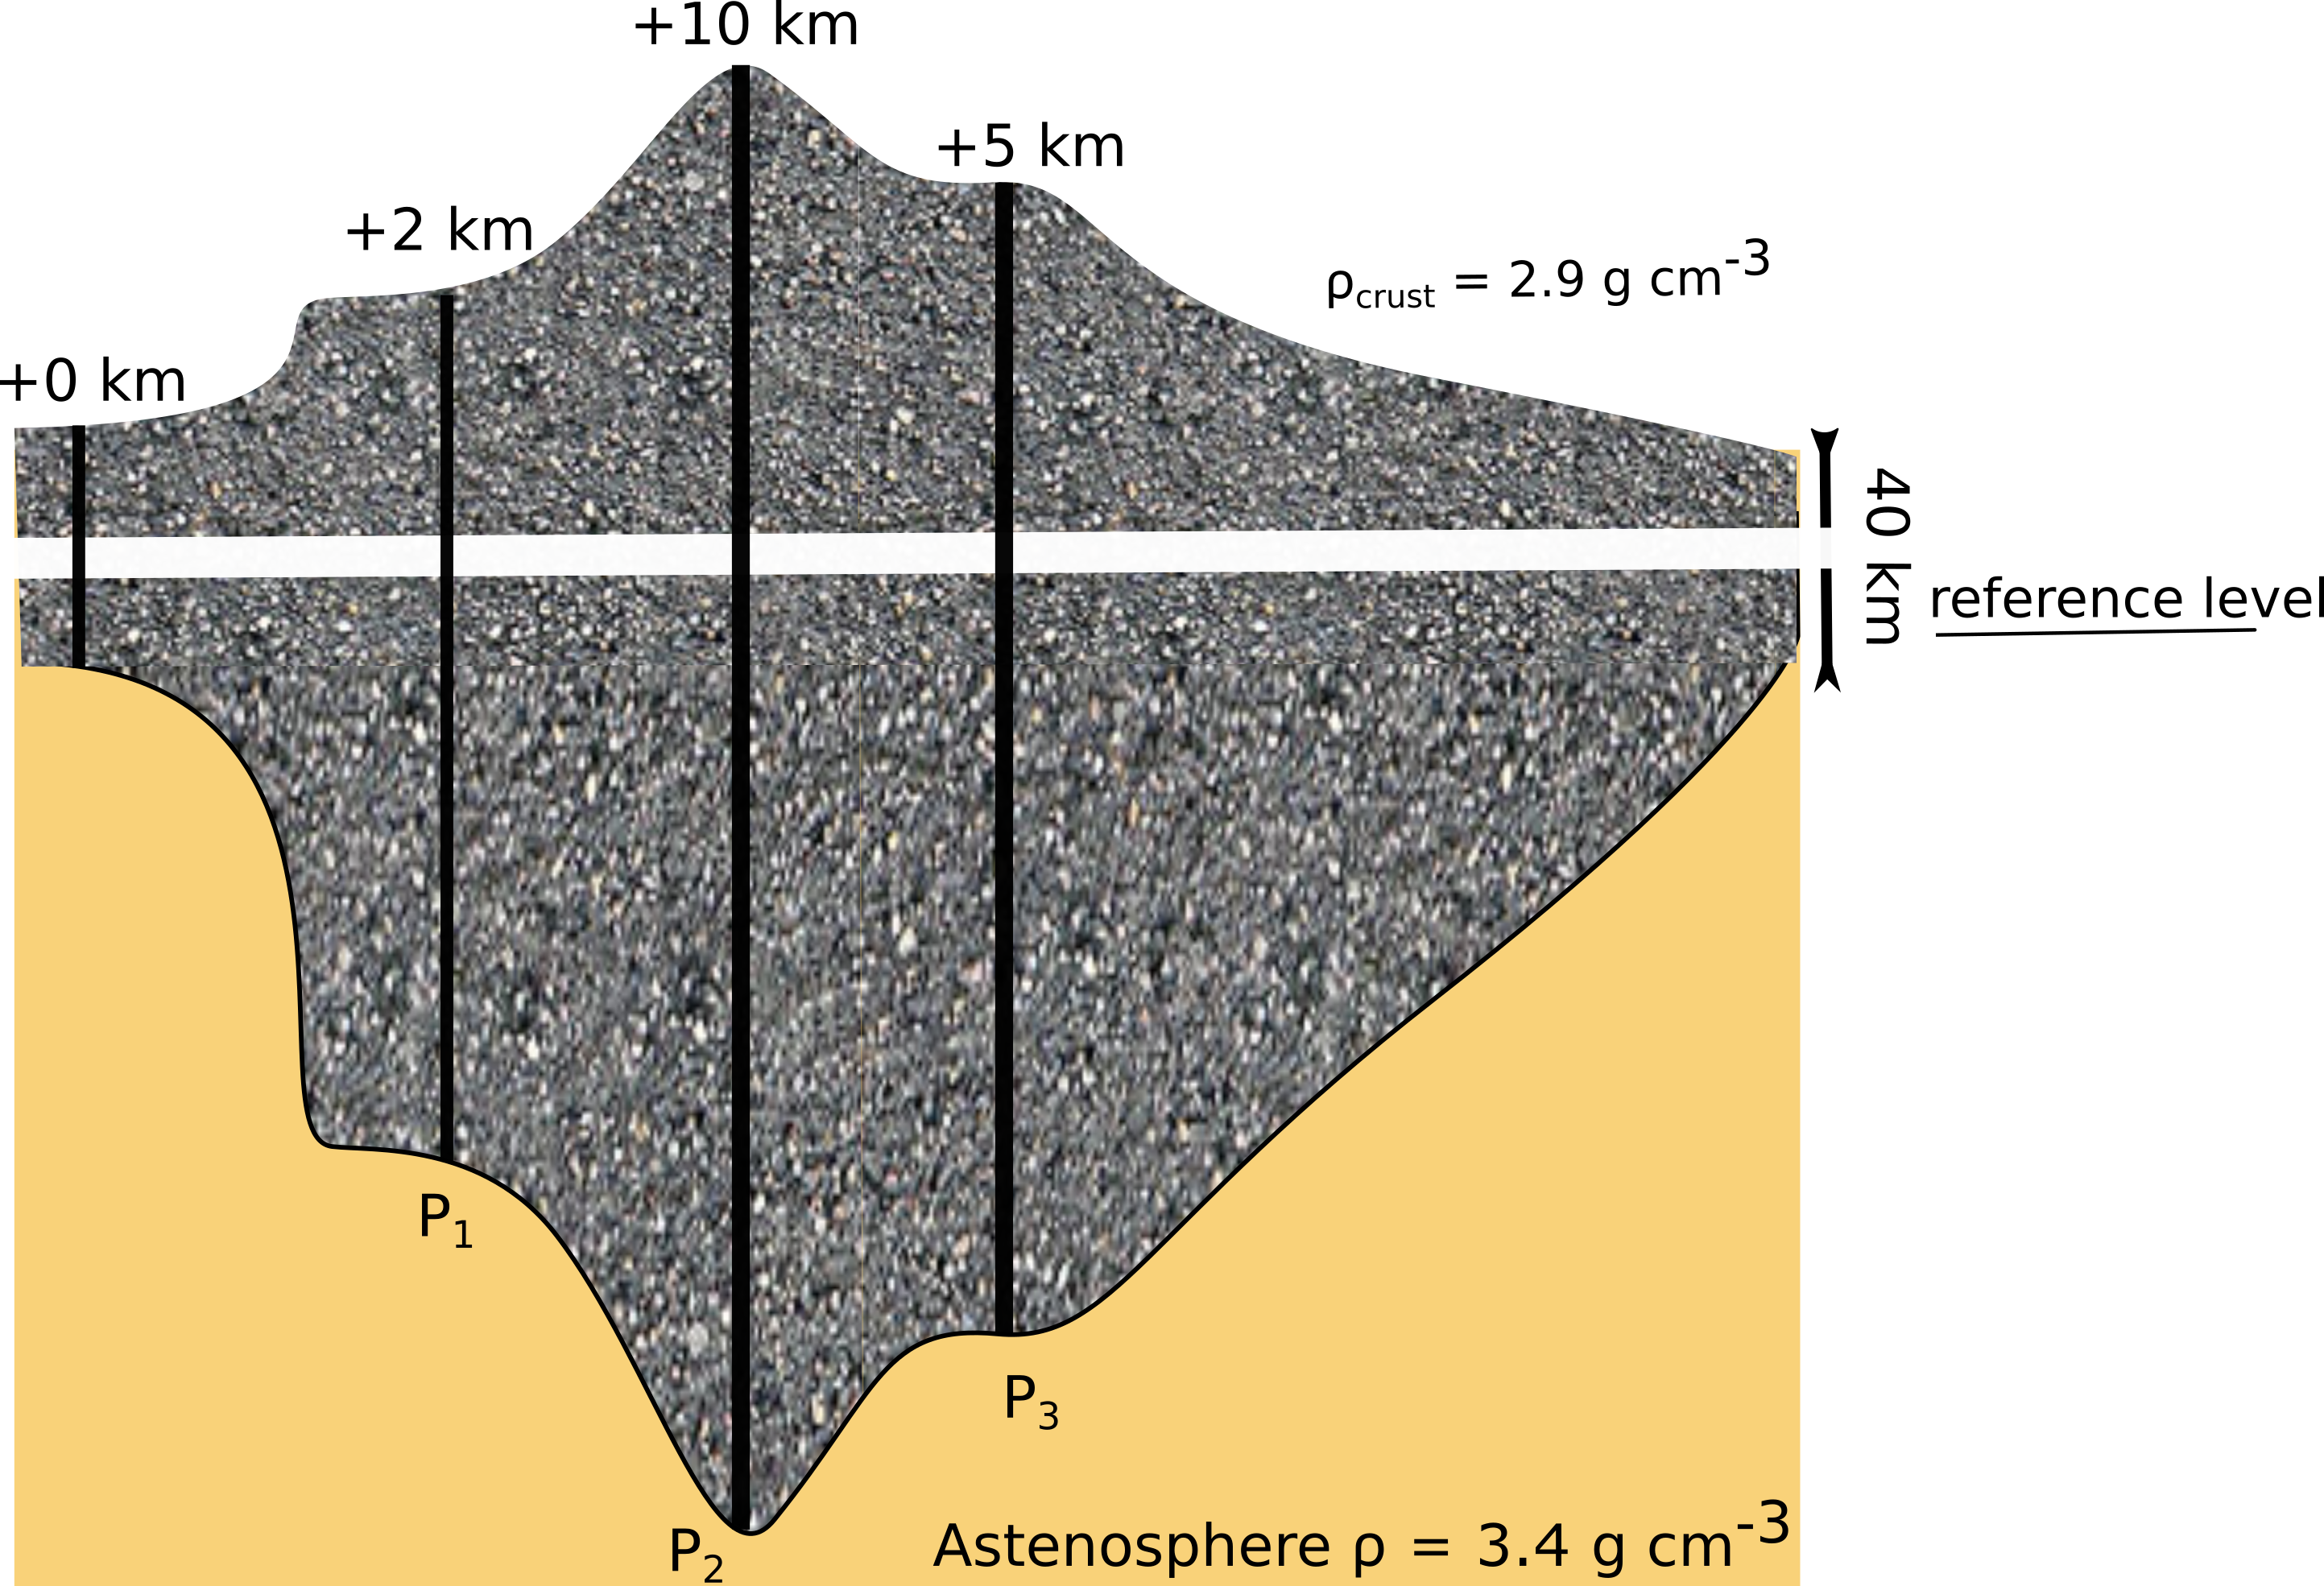
\includegraphics[width=0.5\textwidth]{Figures/Gravimetry/Airy.png}
  \end{center}
The figure above illustrates a crust with a homogenous density and a mountain change floating on the asthenosphere. Consider this as an idealised case in which every vertical slice is locally balanced (i.e. everything is in hydrostatic equilibrium which reduces to an effective 1D problem). Calculate the thickness differences between $P_1 -- P_3$.


\ifanswers
  \begin{tcolorbox}[enhanced jigsaw,breakable,pad at break*=1mm,
    colback=blue!5!white,colframe=babyblueeyes,title=Solutions]
At the depth of $P_1$ we have:
\begin{align*}
\rho_c H_1 + \rho_A H_A &= \rho_c (H_1 + 2) \\
\rightarrow H_A &= 2 \frac{\rho_c}{\rho_A -\rho_c} \approx 11.6 \, \text{km}
\end{align*}
This means thickness at $P_1$ is 40 + 2 + 11.6 = 53.6 km. Equivalent for the other locations.
\end{tcolorbox}
\fi

\textbf{(c)} Draw an approximate profile for the free-air and the Bouger anomalies. How would the free-air anomaly profile change if the mountain change is not in hydrostatic equilibrium? Which conclusions regarding the temporal evolution of the mountain chain would you draw from that? In which areas along this profile do you think is the assumption of local hydrostatic equilibrium most unlikely and how would this be reflected in the free-air anomaly?
\ifanswers
  \begin{tcolorbox}[enhanced jigsaw,breakable,pad at break*=1mm,
    colback=blue!5!white,colframe=babyblueeyes,title=Solutions]
    \begin{center}
    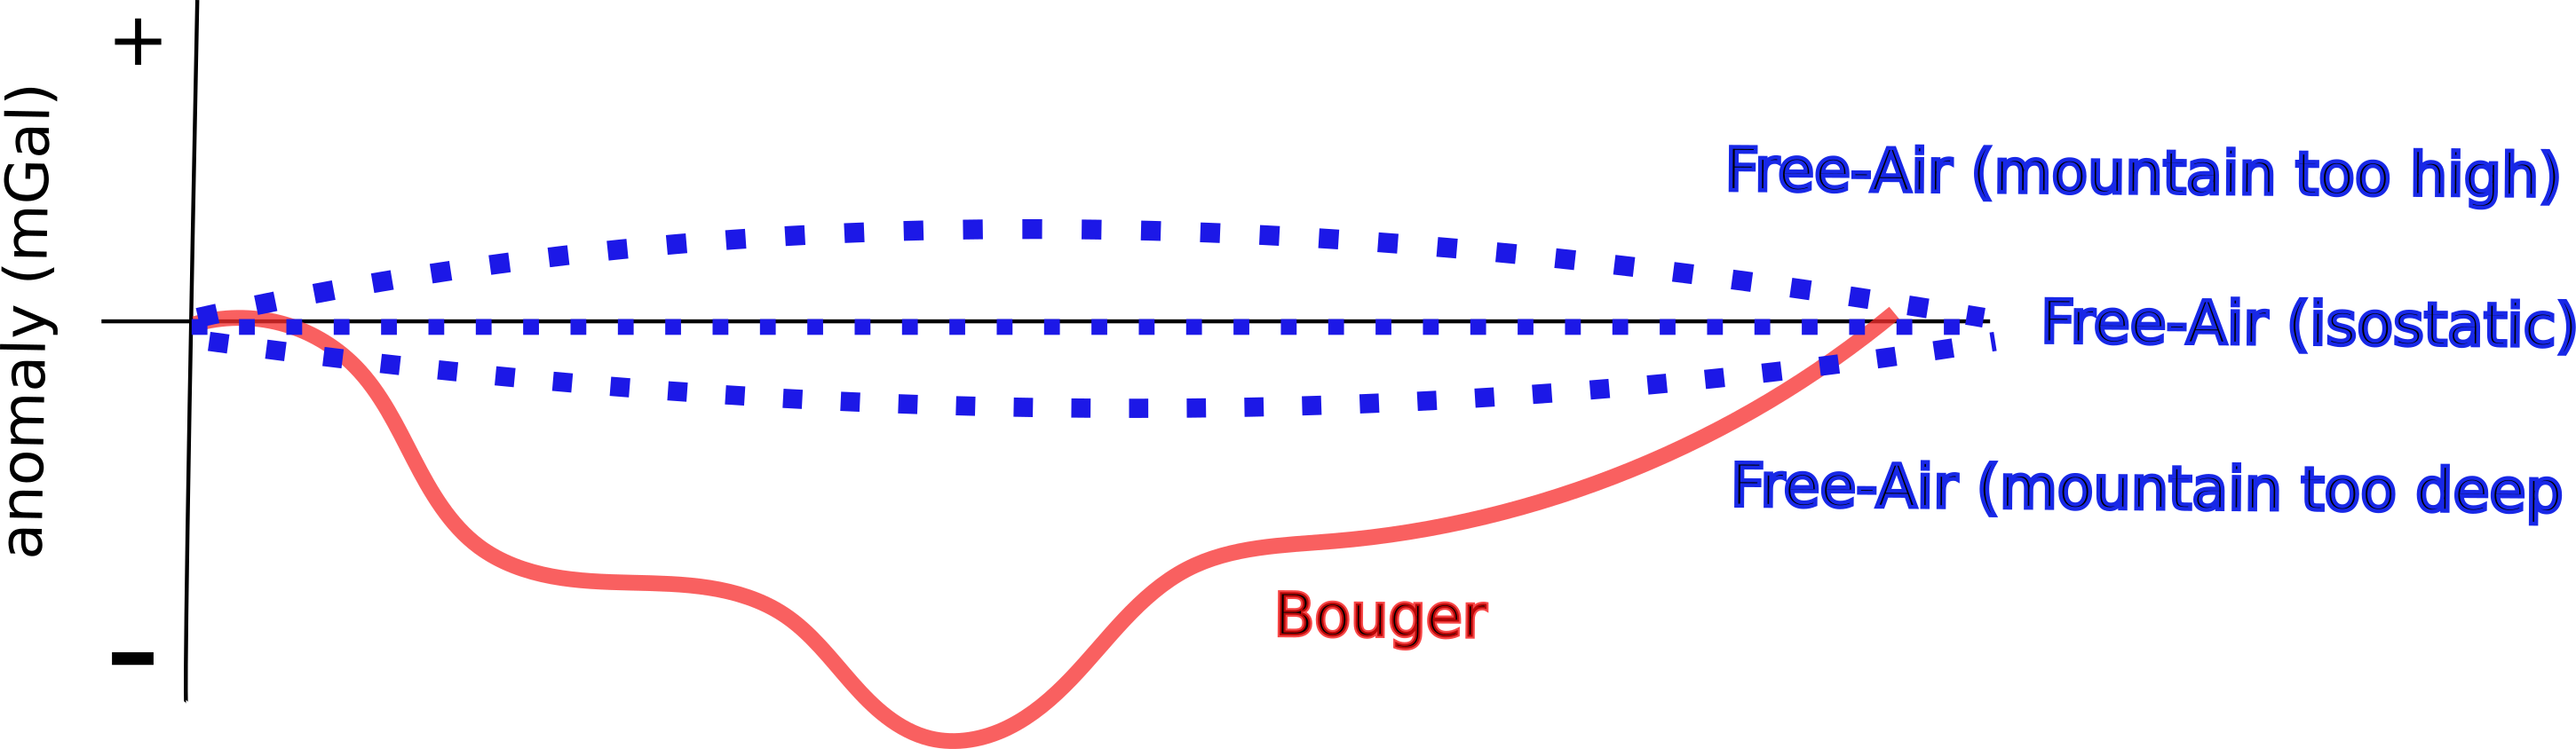
\includegraphics[width=0.9\textwidth]{Figures/Gravimetry/SolutionsProfiles.png}
    \end{center}
    \textbf{Text directly copied from: \href{https://www.geology.cwu.edu/facstaff/tim/TEACHING/Geophysics/gravity_geoid.pdf}{Link2PDF}}
    We can use gravity measurements to determine whether an area is in isostatic equilibrium. If a region is in isostatic equilibrium, there should be no gravity anomaly and hence no excess or lack of mass above the compensation depth. However, in practice, interpreting gravity measurements is a convoluted process. As an example, take the mountains shown above which are in 100\% isostatic compensation of the Airy type. The Bouguer anomaly across these mountains is negative, since below sea level there is a mass deficit under the mountains, ie, the low density root is holding the overlying mountains up. The Bouguer
    anomaly reflects the fact that the overlying mountains have been removed from the correction, which leaves only the mass deficit at depth unaccounted for, which causes the negative Bouguer anomaly. The free air anomaly, on the other hand, will be slightly positive, since this anomaly only takes into account the fact that we’re above sea level in our measurements and doesn’t take into account the distribution of mass below us. The slight positive reading comes from the fact that the overlying mountain is closer to us
    and and our point of measurement than is the compensating low density material at depth, and since gravitational acceleration drops off as $1/r^2$, the closer, mountain attraction io stronger than the more distant lack of attraction due to the mass deficit in the root, which results in a slight positive free air anomaly. The simplest way to determine whether a large-scale structure such as a mountain chain is in isostatic equilibrium is to use the free air anomaly. If a structure is totally compensated, away from the edges of the structure the free air anomaly will be very small. Near the edges is difficult to discern. If the structure is only partially compensated, the or not at all, then the free air anomaly will be strongly positive, up to several hundred millgals, while the Bouguer anomaly will be about zero. Free air anomalies are always almost isostatic anomalies. They do not tell you what type of compensation is ocurring (ie, Pratt versus Airy), but if compensation of any mechanism is complete, then the free air anomaly will be nearly zero.
  \end{tcolorbox}
\fi